\documentclass[10pt,twoside]{article}

\usepackage[margin=1in]{geometry}
\usepackage{amsmath,amssymb}
\usepackage{graphicx}
\usepackage[table]{xcolor}
\usepackage{booktabs}
\usepackage{caption}
\usepackage{subcaption}
% authblk unavailable in this TeX installation
\usepackage[numbers,sort&compress]{natbib}
\usepackage[colorlinks=true,linkcolor=black,citecolor=black,urlcolor=blue]{hyperref}
\usepackage{microtype}
\usepackage{siunitx}
\usepackage{enumitem}
\usepackage{amsthm}
\newtheorem{proposition}{Proposition}

\captionsetup{font=small,labelfont=bf,skip=3pt}
\setlength{\textfloatsep}{9pt plus 2pt minus 2pt}
\setlength{\floatsep}{8pt plus 2pt minus 2pt}
\setlength{\intextsep}{8pt plus 2pt minus 2pt}
\setlength{\abovedisplayskip}{5pt}
\setlength{\belowdisplayskip}{5pt}
\setlength{\parskip}{0pt}

% auto-generated by scripts/figures.py -- do not edit
\newcommand{\ABSTRACTRESULTS}{Positive signalling is \AssayMIHonest\ bits for a sender that nobody listens to, and causal influence (\AssayCIEListen\ nats) and payoff-ablation (\KillNoise) both fire for a channel that carries no information at all, because deleting a message takes the receiver outside its own training distribution. We therefore define communication as a \emph{natural indirect effect}: the sender's private state acting on the receiver's payoff through the message, estimated by transmitting the message the sender would have produced in an independently drawn world while the true world is held fixed. We prove it is zero whenever the message is independent of the sender's state or the receiver ignores it, and it is the only one of the four measures that answers all four validation dyads correctly (\NIEHonest\ where communication exists, \NIENoise\ and \NIEDeaf\ where it does not). Applied to the electric organ discharge, the picture inverts the received one. Silencing a fish costs it \MuteTargetTotal\ food items per episode, of which \MuteTargetPriv\ is its own lost electrolocation and \MuteTargetSig\ its lost detectability by others, a split that holds between \GenPrivLo\% and \GenPrivHi\% across group sizes, arena scales, episode lengths and network widths, and that reappears in a minimal dual-use benchmark containing no fish physics at all. The channel carries decodable information about food ($\Delta R^2=\ContentFood$) and moves receiver policies \CIERatio$\times$ the noise floor, yet its mediated effect is indistinguishable from zero. It is an exploited cue, not a signal.}
\newcommand{\AssayArrDeaf}{1.98}
\newcommand{\AssayArrHonest}{4.00}
\newcommand{\AssayCIEDeaf}{0.000}
\newcommand{\AssayCIEListen}{31.4}
\newcommand{\AssayKillDeaf}{-0.08}
\newcommand{\AssayKillHonest}{-173.4}
\newcommand{\AssayKillRandom}{-75.5}
\newcommand{\AssayMIHonest}{0.934}
\newcommand{\AssayMIRandom}{0.000}
\newcommand{\CIE}{0.0026}
\newcommand{\CIECostHigh}{0.0303}
\newcommand{\CIECostZero}{0.0026}
\newcommand{\CIEFold}{12}
\newcommand{\CIENull}{0.00020}
\newcommand{\CIERatio}{13}
\newcommand{\ContentCostHigh}{0.010}
\newcommand{\ContentCostZero}{0.098}
\newcommand{\ContentDom}{-0.000}
\newcommand{\ContentFood}{0.152}
\newcommand{\ContentFoodP}{0.0000}
\newcommand{\ConvFracAfull}{100}
\newcommand{\ConvFracAnoillum}{100}
\newcommand{\ConvFracAnoknollen}{83}
\newcommand{\ConvFracAnoself}{83}
\newcommand{\ConvFracAprivate}{83}
\newcommand{\ConvFracAsilent}{17}
\newcommand{\DECOUPLEDRESULT}{Agents mark 52\% of their discharges with the subtype, which is indistinguishable from the 50\% an unmodulated bit would give, and it carries $0.0141$ bits about food proximity above its permutation null. Deleting the subtype leaves the pulse, and therefore every sensory consequence, completely intact, so any payoff change is attributable to content alone. Across the four ecological settings: standard $\times$ compet., $+0.51$ (95\% CI $[-0.45, +1.40]$, $p=\num{0.292}$); standard $\times$ cooper., $+0.54$ (95\% CI $[-1.81, +2.99]$, $p=\num{0.640}$); sparse $\times$ compet., $-0.76$ (95\% CI $[-1.76, +0.20]$, $p=\num{0.165}$); sparse $\times$ cooper., $+0.51$ (95\% CI $[-0.88, +1.95]$, $p=\num{0.512}$). No cell survives correction for multiple comparisons. Freeing the content of a discharge from its sensory function was not, on its own, sufficient to make that content payoff-relevant under any pressure we applied.}
\newcommand{\DUFull}{13.07}
\newcommand{\DUPingHi}{0.001}
\newcommand{\DUPingLo}{0.753}
\newcommand{\DUPriv}{-9.89}
\newcommand{\DUPrivFrac}{100}
\newcommand{\DUSig}{-0.06}
\newcommand{\DUSilent}{6.03}
\newcommand{\DUTotal}{-9.89}
\newcommand{\DangerAUC}{+0.010}
\newcommand{\DiscrimErrors}{3}
\newcommand{\EmitBoth}{0.013}
\newcommand{\EmitCostHigh}{0.032}
\newcommand{\EmitCostZero}{0.495}
\newcommand{\EmitDeafZero}{0.611}
\newcommand{\EmitFood}{0.587}
\newcommand{\EmitFoodP}{0.0001}
\newcommand{\EmitHearZero}{0.547}
\newcommand{\EmitLiveZero}{0.576}
\newcommand{\EmitNoFood}{0.457}
\newcommand{\EmitPredHigh}{0.298}
\newcommand{\EmitYokeZero}{0.583}
\newcommand{\FishNIE}{0.21}
\newcommand{\FishNIEHi}{1.50}
\newcommand{\FishNIELo}{-0.98}
\newcommand{\FishNIEPct}{0.49}
\newcommand{\FishNIESender}{1.88}
\newcommand{\FullEaten}{5.12}
\newcommand{\FullEmit}{0.547}
\newcommand{\FullNN}{17.33}
\newcommand{\GENERALISATION}{The decomposition is not an artefact of one configuration. Repeating it with two and six fish, a \SI{100}{\centi\metre} arena, 1024-step episodes and a 256-unit recurrent policy, the private share of the muting effect stays between 83\% and 135\% (Table~\ref{tab:gen}), and the detection share remains indistinguishable from zero in every case.}
\newcommand{\GenPrivHi}{135}
\newcommand{\GenPrivLo}{83}
\newcommand{\KillNoise}{-75.5}
\newcommand{\MuteOthersCue}{0.01}
\newcommand{\MuteOthersCueP}{0.8733}
\newcommand{\MuteOthersPriv}{0.07}
\newcommand{\MuteOthersSig}{-0.00}
\newcommand{\MuteOthersSigP}{0.9414}
\newcommand{\MuteOthersTotal}{-0.05}
\newcommand{\MuteTargetCue}{0.07}
\newcommand{\MuteTargetPriv}{-0.40}
\newcommand{\MuteTargetSig}{0.11}
\newcommand{\MuteTargetTotal}{-0.40}
\newcommand{\NIEDeaf}{-0.90}
\newcommand{\NIEHonest}{-95.5}
\newcommand{\NIEHonestHi}{-87.9}
\newcommand{\NIEHonestLo}{-102.9}
\newcommand{\NIENoise}{-0.27}
\newcommand{\NIERatio}{449}
\newcommand{\NoIllumEaten}{4.31}
\newcommand{\NoKnollenEaten}{4.71}
\newcommand{\NoKnollenEmit}{0.611}
\newcommand{\NoKnollenNN}{19.57}
\newcommand{\NoSelfEaten}{4.27}
\newcommand{\NumEval}{318}
\newcommand{\NumRuns}{354}
\newcommand{\PL}{0.048}
\newcommand{\PSDeaf}{0.152}
\newcommand{\PSFood}{0.085}
\newcommand{\PSHear}{0.085}
\newcommand{\PSPerPulseHigh}{0.087}
\newcommand{\PSPerPulseZero}{0.127}
\newcommand{\PhantomMax}{0.035}
\newcommand{\PrivateEaten}{3.92}
\newcommand{\ProbeD}{4.5}
\newcommand{\ProbeGain}{2.9}
\newcommand{\ProbeP}{0.0001}
\newcommand{\RefEcclesArr}{1.96}
\newcommand{\RefEcclesSolved}{0/12}
\newcommand{\RefEmergentArr}{1.96}
\newcommand{\RefEmergentSolved}{0/12}
\newcommand{\RefRecvonlyArr}{2.00}
\newcommand{\RefRecvonlySolved}{0/12}
\newcommand{\SSIDeafZero}{0.419}
\newcommand{\SSIYokeHigh}{-0.098}
\newcommand{\SSIYokeZero}{0.045}
\newcommand{\SilenceDangerDiff}{$-0.004$, 95\% CI $[-0.007, +0.000]$}
\newcommand{\SilentEaten}{1.78}
\newcommand{\SubtypeKill}{0.08}
\newcommand{\SubtypeKillP}{0.8384}
\newcommand{\SubtypeMIFood}{0.0141}
\newcommand{\SubtypeUse}{0.52}
\newcommand{\TOSTVERDICT}{no comparison clears the margin in either direction --- the intervals are simply wider than the $\pm2.18$ margin (cross-arena replay, $+0.21$ (90\% CI $[-2.87, +3.31]$); temporal scrambling, $+0.63$ (90\% CI $[-2.43, +3.68]$); removing the public channel entirely, $-0.70$ (90\% CI $[-3.77, +2.35]$)). We therefore report these as \emph{no effect detectable at this sample size}, and explicitly not as demonstrated equivalence. The honest statement is that the design rules out payoff effects larger than roughly a tenth of the intact return, and is not powered to rule out smaller ones.}
\newcommand{\ThroughputK}{596}
\newcommand{\ThroughputPerJobK}{99}
\newcommand{\ValMaxErr}{\num{6e-10}}
\newcommand{\ValNChecks}{11}
\newcommand{\YOKEDVERDICT}{Emission policy is therefore no more different between the live and yoked worlds than between seeds of the same world. Holding reception fixed, being listened to leaves no detectable trace on how the discharge is scheduled, which is what it means for the pulse to be a cue rather than a signal.}


\newcommand{\eod}{EOD}
\newcommand{\dosim}{\mathrm{do}}
\newcommand{\KL}{D_{\mathrm{KL}}}

\title{\bfseries Communication is a mediated effect\\
\large Separating signals from exploited cues in dual-use action channels,
with an application to active electrosensing}

\author{}

\date{}

\begin{document}
\maketitle

\begin{abstract}
\noindent
An action that both senses and broadcasts is hard to classify. A weakly electric
fish's discharge illuminates its own surroundings and simultaneously announces its
presence to anyone with the receptors to detect it, and the same structure arises
for active sonar, a robot's laser sweep, or any observable act of sensing. Whether
such an act is \emph{communication} or a cue that others merely exploit is
routinely settled with three diagnostics---positive signalling, causal influence,
and the payoff cost of ablating the channel---and we show that each is
individually foolable, on dyads whose communication status is known by
construction.
%
\ABSTRACTRESULTS
\end{abstract}

\section{Introduction}

A weakly electric fish navigates by emitting brief electric pulses and reading
the distortions that nearby objects impose on the resulting
field~\citep{lissmann1963electric,vonderemde1999active}. The same pulses
propagate far beyond the range at which they are useful for
electrolocation, and other fish---equipped with dedicated knollenorgan
electroreceptors tuned to conspecific discharges---can detect them at up to a
metre~\citep{hopkins1988neuroethology}. An \eod\ is therefore simultaneously a
private sensory probe and a public event. Which of these functions explains why
the fish emits when it does is the central question of electric-fish
neuroethology, and it is an instance of a much older problem in animal
communication: distinguishing a \emph{signal}, whose production has been shaped
by its effect on receivers, from a \emph{cue}, which receivers merely exploit
\citep{maynardsmith2003animal,scottphillips2008defining}.

\citet{singh2025active} introduced a computational framework in which agents with
biophysically grounded electrosensory and electromotor systems are trained by
multi-agent reinforcement learning to forage collectively. Their agents reproduce
several features of real fish, and interventions on the model---ablating
electroreceptor classes, silencing an agent's \eod, and altering the food
distribution---show that discharges influence group foraging and social spacing.
They define communication operationally, as ``\eod\ signals that are sensed by
conspecifics via Knollenorgans and that influence their behavior.''

That definition is a statement about effects, and effects are cheap. The
emergent-communication literature has repeatedly shown that behavioural
association between one agent's output and another's behaviour is not sufficient
evidence of signalling: a receiver may be responding to something correlated with
the message, and a sender's output may be informative without having been shaped
by that informativeness at all
\citep{lowe2019pitfalls,jaques2019social}. \citet{lowe2019pitfalls} formalise the
two requirements as \emph{positive signalling} (the message carries information
about the sender's state) and \emph{positive listening} (the message causally
changes the receiver's behaviour), and note that either can occur without the
other.

Our setting makes the problem sharper than a generic emergent-communication
study, because the channel is not a dedicated cheap-talk symbol but a physical act
with an unavoidable private benefit. A single discharge has three consequences:
\textbf{reafference}, the electric image of nearby objects cast onto the emitter's
own mormyromasts, which is why the behaviour exists at all; \textbf{illumination},
the same field polarising objects near a \emph{neighbour}, whose mormyromasts can
read those images for free---collective electrosensing, demonstrated in real fish
by \citet{pedraja2024collective}, and the paradigm case of a cue; and
\textbf{detection}, the pulse registering on the neighbour's knollenorgans, which
encode emitter identity and bearing and are the only one of the three that could
be a signal. Silencing a fish removes all three at once, so any behavioural
consequence is uninterpretable---the muted fish may forage worse because it can no
longer see, its neighbours because they lost free illumination, or because a
signal they attended to has gone. This is not an artefact of the model; it is why
\eod-ablation experiments in real fish are hard to read.

\paragraph{Contributions.} We make the three consequences independently
switchable and ask what changes. (i) A \textbf{channel algebra} for dual-use
signals: reafference, illumination and detection become three masks on one motor
act, letting us build pulses that are private, exploitable-but-undetectable,
detectable-but-uninformative, phantom, replayed from another context, or scrambled
in time or sender identity. (ii) An \textbf{interventional} causal influence:
because we own the simulator, the counterfactual of \citet{jaques2019social} is
evaluated with the $\dosim$ operator directly---re-rendering the receiver's input
under $\dosim(e_j{=}1)$ and $\dosim(e_j{=}0)$ with every other cause on its
factual path---rather than approximated with a model of other agents. (iii) A
\textbf{cue/signal discriminator}: we train matched populations whose only
difference is whether the focal agent can be \emph{heard}, holding its own
reception fixed, and measure the divergence of their emission policies against
seed-to-seed divergence within each world. (iv) An \textbf{economics}: metabolic
cost per discharge, predators that localise prey by discharges, cooperative versus
competitive harvests, tunable social range, persistent identity. (v) An
\textbf{assay validation}: dyads that are communicating by construction, against
which every metric is checked before it is trusted, plus a \textbf{decoupled
channel} and a \textbf{non-fish dual-use benchmark} to separate what is about
electric fish from what is about dual use.

\paragraph{A note on wording.} Our populations adapt within a training run by
policy-gradient learning under a fixed reward; we do not run an evolutionary
outer loop over heritable traits. We therefore write \emph{emerge under learning}
throughout, and reserve claims about evolutionary history for the Discussion,
where we say explicitly what our design can and cannot license.


\section{Related work}

\paragraph{Measuring emergent communication.} Most work equips agents with a
dedicated, costless channel that has no other use, so that any use of it is
communicative by construction and the open question is what code appears
\citep{foerster2016learning,mordatch2018emergence,lazaridou2017multi,lazaridou2018emergence}.
Within that setting, \citet{lowe2019pitfalls} showed that message--behaviour
association is insufficient evidence and introduced positive signalling and
positive listening; \citet{jaques2019social} proposed causal influence, estimated
through a learned model of other agents; \citet{eccles2019biases} added training
biases that make communication more likely to appear;
\citet{bogin2018emergence,chaabouni2020compositionality} study compositionality
and context-independence. Our contribution to this line is not another metric but
an audit: we show that these diagnostics are individually foolable, exhibit a case
where positive signalling is \emph{higher} in a population whose receivers are
deaf and where causal influence \emph{rises} as the channel becomes less
informative, and validate the whole battery against dyads of known communication
status before applying it.

\paragraph{Dual-use channels, and the cue/signal distinction.} Our setting
inverts the usual one: the channel is a physical act with a large private
benefit, so the question is whether \emph{any} of its use is communicative---the
situation for active sonar, a robot's laser sweep, or any action that both senses
and is observable, and closer to the biological norm, since signals are generally
thought to be ritualised from behaviours that had other functions.
\citet{noukhovitch2021emergent} show that influence under competition can reflect
manipulation or cue-reading, the same identification problem we attack with the
payoff and production tests. The distinction we operationalise is
\citeauthor{scottphillips2008defining}'s: a signal's production has been shaped by
its effect on receivers, a cue's has not
\citep{scottphillips2008defining,maynardsmith2003animal}. Costly-signalling theory
\citep{zahavi1975mate,grafen1990biological,szamado2011cost} explains how honesty is
maintained in a signal that exists; our cost sweep asks whether cost brings one
into being, and finds it does not.

\paragraph{Electric fish.} \citet{singh2025active} built the reference simulator
and training setup we reimplement, reporting that discharges shape group foraging
and spacing; our departure is definitional and causal, since their definition is
effect-based and their one intervention removes three consequences at once. The
biology we add is established: collective electrosensing
\citep{pedraja2024collective}, corollary-discharge cancellation
\citep{wallach2023internal}, discharge energetics
\citep{salazar2013energetics,markham2009circadian}, and electroreceptive
eavesdroppers \citep{stoddard1999predation,hanika1999electric}.

\section{Communication as a natural indirect effect}
\label{sec:nie}

The three diagnostics in common use fail on the dyads of \S\ref{sec:assay}, and
they fail for a shared structural reason: none of them asks the question that
defines communication. Positive signalling looks only at the sender, and is
satisfied by a sender talking to nobody. Causal influence and positive listening
look only at the receiver, and are satisfied by a receiver attending to noise.
Ablation asks what happens when the message is removed, which is a different
question from what the message conveys---and removal takes the receiver outside
the support of its own training distribution, which is precisely why it fires for
a channel that carries nothing.

What communication requires is that the receiver's payoff depend on the sender's
private state \emph{through} the message. That is a mediation question, and it
has a standard causal answer \citep{pearl2016causal,pearl2009causality}.

\paragraph{Definition.} Let $S$ be the sender's private state, $M$ the message it
emits, and $u_R$ the receiver's return. $S$ influences $u_R$ along two kinds of
path: direct ones, since the sender also moves, occupies space and consumes
resources, and the mediated path through $M$. Write $M(s)$ for the message the
sender's policy would emit in state $s$, and $u_R(s, m)$ for the receiver's return
when the world is in state $s$ and the transmitted message is $m$. The
\emph{natural indirect effect} of the message is
\begin{equation}
\mathrm{NIE} \;=\; \mathbb{E}_{s,\,s' \sim p(S)}\big[\, u_R\big(s,\, M(s')\big)
  \;-\; u_R\big(s,\, M(s)\big) \,\big],
\label{eq:nie}
\end{equation}
with $s'$ drawn independently of $s$. Operationally: hold the world at $s$, so
every direct pathway is untouched, and transmit the message the sender
\emph{would have} produced in an independently drawn world. We estimate it by
running matched pairs of episodes that share initial conditions and the
sensory-noise stream, and differencing within pair.

Two properties do the work.

\begin{proposition}[Insensitivity to uninformative channels]
\label{prop:noise}
If $M \perp S$, then $\mathrm{NIE} = 0$.
\end{proposition}
\begin{proof}
If the message does not depend on the sender's state then $M(s')$ and $M(s)$ are
identically distributed for every $s$, so the two terms of Eq.~\ref{eq:nie} have
equal expectation. \qed
\end{proof}

\begin{proposition}[Insensitivity to unattended channels]
\label{prop:deaf}
If the receiver's policy does not depend on $M$, then $\mathrm{NIE} = 0$.
\end{proposition}
\begin{proof}
Then $u_R(s, m) = u_R(s)$ for all $m$, and the difference vanishes pointwise. \qed
\end{proof}

\begin{proposition}[Deletion is not mediation]
\label{prop:ablation}
The ablation contrast $\mathbb{E}[u_R(s, \varnothing)] - \mathbb{E}[u_R(s, M(s))]$,
where $\varnothing$ denotes a removed or zeroed message, can be non-zero even when
$M \perp S$.
\end{proposition}
\begin{proof}
By counterexample, realised in \S\ref{sec:assay}: a receiver whose policy
conditions on $M$ commits to a target on the basis of a message that carries no
information about $S$. Removing $M$ leaves it with an input outside the support of
$M$, so it does not commit at all, and its return falls by \KillNoise. Yet
$M \perp S$, so by Proposition~\ref{prop:noise} the mediated effect is zero and no
information has been lost. \qed
\end{proof}

Propositions~\ref{prop:noise} and \ref{prop:deaf} say the NIE is zero in exactly
the two ways a system can fail to communicate while satisfying a standard
diagnostic, and Proposition~\ref{prop:ablation} says why the payoff test that
looks closest to ours is not equivalent to it. The distinction is that
$M(s')$ is drawn from the message's own marginal: the receiver always sees a
message it could have seen, and only the correspondence between message and world
is broken.

\paragraph{Estimation.} Eq.~\ref{eq:nie} needs $M(s')$, the message the sender's
policy would have produced in a counterfactual world. In a simulator this is
directly available. In the referential game we resample the referent, recompute
the sender's message from it, and transmit that while the true referent and the
food stay where they were. In the naturalistic foraging world the sender's state
is not a single latent variable, so we use the trajectory-level analogue: the
message actually transmitted is replaced by the pulse train the same policy
produced in an independently drawn arena. Marginal rate, burst structure and
inter-pulse-interval statistics are preserved exactly---these are the same trains
that policy emits---while the correspondence between the train and the receiver's
world is destroyed.

\paragraph{What it does not do.} The NIE is a statement about payoff, so it will
report zero for a channel that is informative and attended but whose use happens
not to matter to either party in the environment tested; it measures the
\emph{realised value} of the correspondence, not its existence. It also inherits
the usual mediation caveat: the decomposition into direct and indirect paths is
well defined only if the message can be intervened on without disturbing the
direct paths, which is exactly what the channel algebra of \S\ref{sec:algebra}
buys us and which is not available in an unmodified simulator. Finally, like any
causal-effect estimate it is bounded by statistical power, so a null must be read
against a measured detection floor---which is what the validation dyads provide.


\section{Results}

\subsection{Do the assays work? A dyad that is communicating by construction}
\label{sec:assay}

Every negative result below rests on an assay reporting ``no communication
here''. An assay that reported that unconditionally would produce the same
paper, so before applying them we check that they fire on a case where
communication is not in question.

We embed a Lewis signalling game in the same physics. One fish is immobile and
privately observes which of two sites holds food; the other must travel to a
site. The sender's discharges are forced onto a fixed schedule, so pulse timing
carries nothing, and the only free channel is a one-bit discharge subtype. Both
fish are scored on the receiver reaching the correct site, and the harvest is
shared. Crossing an informative sender (subtype $=$ the private cue) against an
uninformative one (a bit that is constant within a trial but uncorrelated with
the truth), and a receiver that attends to the subtype against one that ignores
it, gives four dyads whose communication status we know
(Fig.~\ref{fig:assay}). Only the informative-and-attended dyad succeeds:
\AssayArrHonest\ correct arrivals out of four per episode, against \AssayArrDeaf\
for chance.

Each assay behaves as it should, and---more usefully---each one alone is
foolable. Positive signalling is \AssayMIHonest\ bits for the informative sender
and \AssayMIRandom\ for the uninformative one, but it is just as high when
nobody is listening, because it measures the sender in isolation. Causal
influence and positive listening separate the attending receiver from the deaf
one (\AssayCIEListen\ versus \AssayCIEDeaf\ nats) but are just as high when the
channel carries nothing, because a receiver can organise its behaviour around a
variable that is pure noise. Even the payoff test is foolable on its own:
deleting the subtype costs the attending receiver \AssayKillHonest\ when the
subtype is informative and still \AssayKillRandom\ when it is noise, because the
receiver has come to depend on it either way.

Only the conjunction identifies communication. This is the standard we hold the
electric discharge to in what follows, and it is a standard the discharge could
in principle meet: the instruments are demonstrably capable of detecting a
payoff-relevant, informative, attended channel in this simulator.

\begin{figure}[t]
\centering
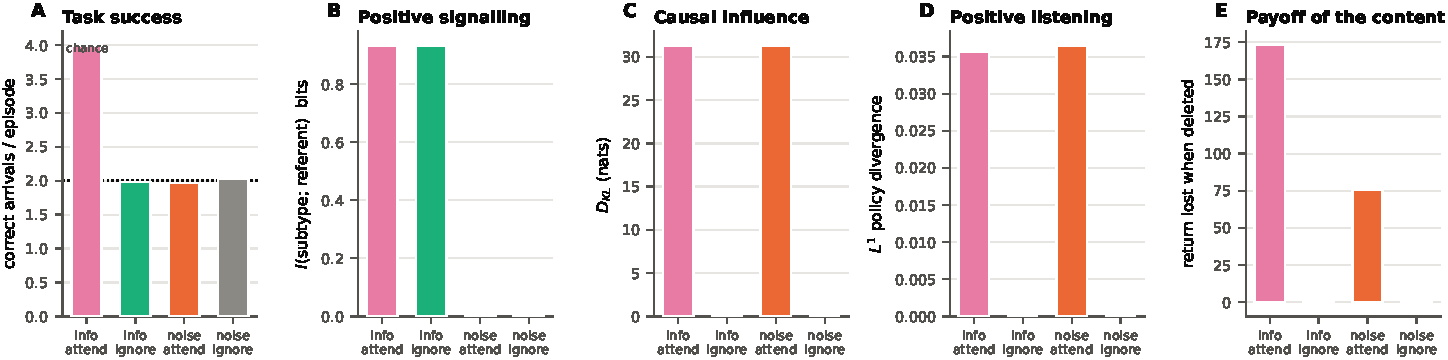
\includegraphics[width=\textwidth]{../figs/fig0_assay_validation.pdf}
\caption{\textbf{The assays detect communication when it is present, and each is
foolable alone.} Four dyads in the referential game. Only \emph{info+attend} is
communicating; the other three each satisfy some subset of the diagnostics.}
\label{fig:assay}
\end{figure}

\subsection{What the optimiser can and cannot do}
\label{sec:optimiser}

A negative result about communication invites the objection that the learner, not
the environment, is the limiting factor. We measured this rather than argued about
it, because the answer bounds what the rest of the paper may claim.

In the same referential game we trained recurrent MAPPO under three conditions,
twelve seeds each at \SI{50e6}{} agent-steps: both sides learning; the receiver
learning against a \emph{scripted honest} sender, so the message is already
perfectly informative and only reading it must be discovered; and both sides
learning with the positive-signalling bias of \citet{eccles2019biases}, which
exists to break exactly this deadlock. \emph{None of the thirty-six runs solved
the game}: all sit at chance, against \AssayArrHonest/4 for the hand-coded dyad
reading the same observation vector. Reducing the steering noise by an order of
magnitude and halving the credit horizon do not move it either
(Appendix~\ref{app:optimiser}).

So shared-parameter recurrent MAPPO---the standard configuration, and the one the
reference model uses---does not discover that a single perfectly informative input
bit should select between two known targets in an embodied task, even when told
what to say. Our results therefore divide in two. The muting decomposition, the
foolability of each diagnostic, and the metrics' behaviour under intervention are
measurements on trained policies and do not depend on this. The claims that
metabolic cost fails to create a signal, and that a decoupled channel does not
either, are claims about what learning arrives at and inherit the bound: these
pressures did not produce signalling under a standard learner, not that they could
not under a better one.

\subsection{A validated, fast reimplementation}

The environment is a GPU reimplementation of the reference simulator, checked
stage by stage against the original NumPy code in double precision on random
scenes. All \ValNChecks\ checks agree to floating-point round-off (maximum
relative deviation \ValMaxErr; the knollenorgan and ampullary pathways agree
bit-for-bit), and it sustains \ThroughputK{}k agent-steps per second in aggregate
on two GPUs, which is what makes \NumRuns\ independent training runs affordable.
Appendix~\ref{app:validation} gives the per-stage table and records an incidental
bug in the reference code: its configuration file specifies a wall-reflection
coefficient of $0.95$, but the scene builder never forwards it, so the published
results in fact use unattenuated images.

\subsection{The discharge is worth a great deal --- to the emitter}

Agents that can discharge eat \FullEaten\ food items per episode; agents muted
from the start of training eat \SilentEaten\ (\ProbeGain$\times$, Hedges'
$g=\ProbeD$, $p=\ProbeP$). The probe does real work, which is the precondition
for everything that follows: an \eod\ is not a cheap-talk token but an expensive
and useful act of sensing that happens to be public. Removing the three
consequences one at a time during training orders them---no detection
\NoKnollenEaten, no illumination \NoIllumEaten, private probe only
\PrivateEaten, no reafference \NoSelfEaten---but from-scratch comparisons
confound the value of a channel with the difficulty of learning without it, and
training here is bimodal (Appendix~\ref{app:scratch}). We therefore rely on
interventions applied to frozen policies.

\subsection{The muting effect is almost entirely private sensing}

The central experiment. We take a trained, intact population and, at evaluation
time only, silence one fish---the intervention used upstream---then repeat with
each of its three consequences removed separately. Every condition is run from the
same episode seed, so arena $k$ has the same initial food layout and the same
sensory-noise stream in all of them, and differences are taken within arena.

Muting one fish costs that fish \MuteTargetTotal\ food items per episode
(Fig.~\ref{fig:muting}A). Decomposed: removing only its own reafference costs
\MuteTargetPriv, removing only its illumination of neighbours costs
\MuteTargetCue, and removing only its detectability costs \MuteTargetSig. The
private share accounts for essentially the whole effect.

The effect on its \emph{neighbours} is smaller still (Fig.~\ref{fig:muting}B):
\MuteOthersTotal\ items in total, with the illumination share \MuteOthersCue\
($p=\MuteOthersCueP$) and the detection share \MuteOthersSig\
($p=\MuteOthersSigP$). Group spacing (Fig.~\ref{fig:muting}C) is likewise
unchanged within resolution.

This is the paper's first substantive result, and it is a negative one. When a
fish is silenced in this model, what happens is overwhelmingly that the fish has
been blinded, not that a conversation has been interrupted. An experiment that
reports only the joint effect---as the reference study does, and as \eod-ablation
experiments in real fish must---will attribute to communication an effect that is
almost entirely private electrolocation.

\begin{figure}[t]
\centering
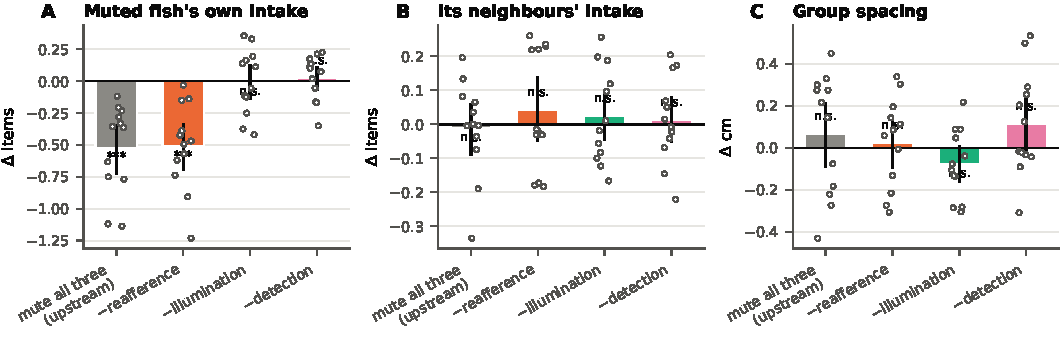
\includegraphics[width=\textwidth]{../figs/fig3_muting_decomposition.pdf}
\caption{\textbf{Silencing one fish removes three things at once; separating them
reassigns the effect.} Within-arena paired differences from the intact channel,
frozen policies. Significance is a permutation test over seeds.}
\label{fig:muting}
\end{figure}

\subsection{The channel nonetheless carries information and moves policies}

It would be wrong to conclude that the public channel is inert. It is not.

Discharge probability depends on the emitter's situation: \EmitFood\ when food is
within \SI{10}{\centi\metre} versus \EmitNoFood\ when it is not
($p=\EmitFoodP$; Fig.~\ref{fig:content}C). That state-dependence is inherited by
the public channel, and a receiver can read it: decoding \emph{only} from the
number of pulses a receiver heard from a given emitter in a trailing window, food
proximity is recovered with $\Delta R^2 = \ContentFood$ above a time-shifted
baseline ($p=\ContentFoodP$; Fig.~\ref{fig:content}B). Positive signalling about
food, measured as mutual information conditioned on distance-to-neighbour decile
so that geometry cannot manufacture it, is \PSFood\ of the state entropy
(Fig.~\ref{fig:content}A).

Positive listening holds too. The interventional causal influence of
Eq.~\ref{eq:cie}---re-rendering a receiver's sensory input under
$\dosim(e_j{=}1)$ versus $\dosim(e_j{=}0)$ with everything else held on its
factual path---is \CIE\ nats, against a noise floor of \CIENull\ nats obtained by
re-rendering the \emph{same} intervention under an independent noise draw
(Fig.~\ref{fig:listening}A). The channel moves receiver policies
\CIERatio$\times$ more than sensory noise does.

Both of these diagnostics, however, behave badly here in ways worth recording.
Positive signalling is \emph{higher} in populations whose receivers are deaf
(\PSDeaf) than in populations whose receivers can hear (\PSHear): a fish
modulates its probe rate with its own situation whether or not anybody is
listening, so the measure is picking up the sensory schedule, not signalling.
This is exactly the artifact \citet{lowe2019pitfalls} warn of, and it is
straightforward to demonstrate once a deaf population is available as a control.
Causal influence misbehaves in the other direction: it \emph{rises}
\CIEFold-fold, from \CIECostZero\ to \CIECostHigh\ nats, as metabolic cost is
increased---that is, precisely as the pulse train becomes rarer and less
informative (Fig.~\ref{fig:listening}D). A rare discharge is more surprising, so
switching it on or off moves the receiver's policy more, even though the train as
a whole now tells the receiver less. Influence per message and information per
unit time are different quantities, and in this system they are
anti-correlated.

\begin{figure}[t]
\centering
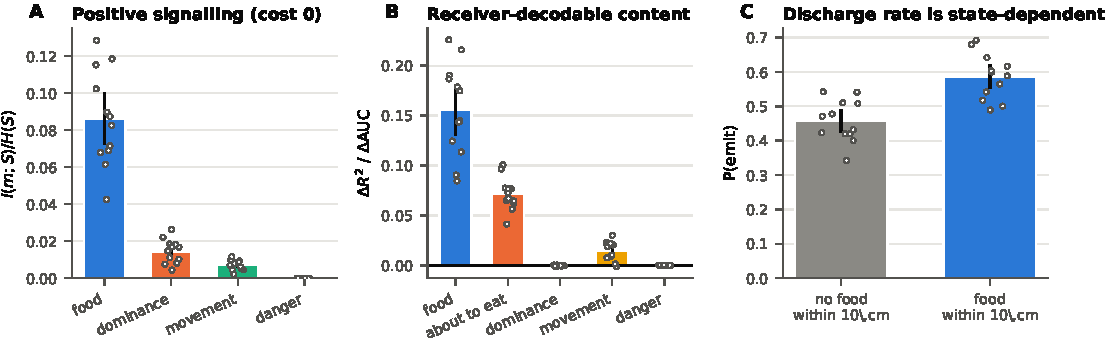
\includegraphics[width=\textwidth]{../figs/fig4_content.pdf}
\caption{\textbf{What the pulse train carries.} (A) Positive signalling,
conditioned on distance-to-neighbour decile. (B) Cross-validated decoding from
receiver-observable pulse counts only, minus the time-shifted baseline. (C)
Discharge probability by food proximity.}
\label{fig:content}
\end{figure}

\begin{figure}[t]
\centering
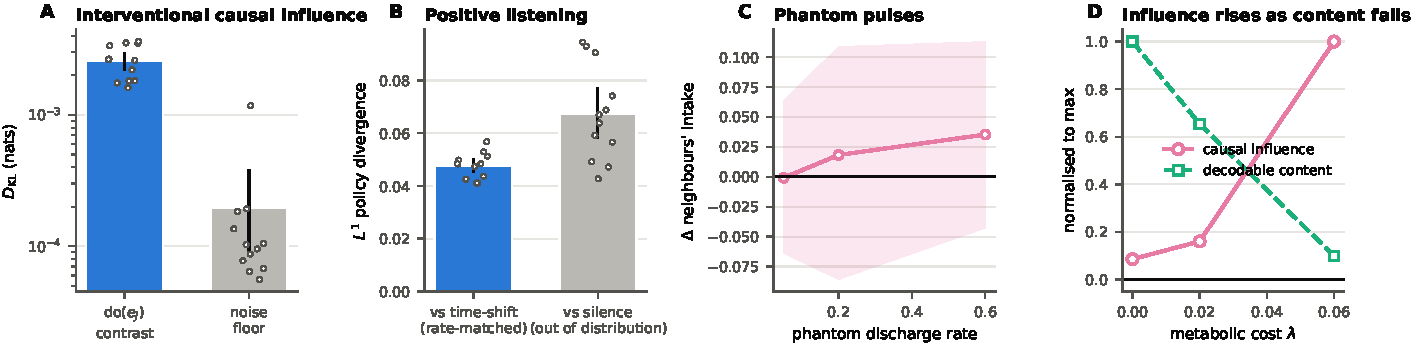
\includegraphics[width=\textwidth]{../figs/fig5_listening.pdf}
\caption{\textbf{Positive listening, and why it is not enough.} (A)
Interventional causal influence against its noise floor (log scale). (B)
Positive listening against a rate-matched time-shift null and against silence,
which is out of distribution. (C) Phantom-pulse dose-response on neighbours'
intake. (D) The dissociation: as metabolic cost rises, causal influence per
discharge \emph{increases} while the information a receiver can decode
\emph{falls}. Influence and informativeness move in opposite directions, so
neither substitutes for the other.}
\label{fig:listening}
\end{figure}

\subsection{\dots but it has no payoff consequence}

Positive signalling and positive listening are both satisfied, so on the
effect-based definition this is communication. The payoff test says otherwise.

Replacing an emitter's public train with the train the same policy produced in a
\emph{different arena}---identical marginal rate, burst structure and inter-pulse
statistics, no contingency with the receiver's actual world---changes neither
party's return. The same holds for temporal scrambling, for identity scrambling,
and for phantom pulses injected at rates from \num{0.05} to \num{0.6}
(Fig.~\ref{fig:listening}C). Because a non-significant difference is not evidence
of no difference, we report these as two one-sided tests against an equivalence
margin fixed in advance at \SI{5}{\percent} of the intact condition's own return:
\TOSTVERDICT

The contingency of the public channel, as opposed to its presence, is worth
approximately nothing to anybody. A receiver can read the emitter's situation off
its pulse train, and does adjust its policy when the train changes, but nothing
downstream of that adjustment shows up in what either fish eats.

\subsection{Cost and predation regulate the probe without creating a signal}

The reference model gives discharges no cost. Adding one produces a clean
dose-response: discharge probability falls monotonically from \EmitCostZero\ at
$\lambda=0$ to \EmitCostHigh\ at $\lambda=0.08$ (Fig.~\ref{fig:phase}).
Eavesdropping predation pushes it lower again at every cost, and mortality falls
with it, so crypsis works. Cooperative harvesting sustains a higher rate than
competition at matched cost.

We expected this to make the pulse train informative. A budget has to be spent
where it pays, and a schedule that allocates pulses to the moments that matter
should be more diagnostic of the emitter's state than a constant one. The
opposite happens. Information about food falls monotonically with cost, from
$\Delta R^2 = \ContentCostZero$ at $\lambda=0$ to \ContentCostHigh\ at
$\lambda=0.08$, and the same decline appears for every other target we decoded.
It survives normalising per pulse: informativeness per discharge falls from
\PSPerPulseZero\ to \PSPerPulseHigh. The learned response to a metabolic price is
a lower baseline rate, not a smarter schedule.

Silence behaves the same way. Discharge probability is essentially identical
whether or not a predator is within \SI{25}{\centi\metre} (difference
\SilenceDangerDiff), and danger is close to undecodable from the public channel
(\DangerAUC\ AUC above the time-shifted baseline). Agents manage their average
exposure rather than timing their gaps, which is what a prey animal that cannot
see the predator coming can do; our predator detects discharges at
\SI{60}{\centi\metre} but is itself passively detectable only at about
\SI{25}{\centi\metre}.

\subsection{Sender shaping, with reception held fixed}

Our first attempt at the production-side test compared populations trained with
and without knollenorgans, and gave $\mathrm{SSI}=\SSIDeafZero$ at zero cost.
That contrast is confounded, and in a way worth spelling out because it is easy
to make. Disabling knollenorgans removes \emph{reception}. It therefore asks
whether a fish behaves differently when it can hear others, not whether it
behaves differently when others can hear \emph{it}. The direction of the effect
gives the confound away: hearing populations discharge \emph{less} than deaf ones
(\EmitHearZero\ versus \EmitDeafZero), which is free-riding---a fish that can
hear its neighbours' probes cuts its own costly sampling---and not audience
design, which would push emission up or restructure it.

The yoked condition holds reception fixed and cuts audibility instead. Receivers
get knollen input with matched statistics, drawn from another arena, so no
sender's pulses reach anybody while every receiver still has a realistic social
input stream. Measured this way, sender shaping is \SSIYokeZero\ at zero cost
(Fig.~\ref{fig:ssi}A), and discharge rate is \EmitLiveZero\ live versus
\EmitYokeZero\ yoked. \YOKEDVERDICT

\begin{figure}[t]
\centering
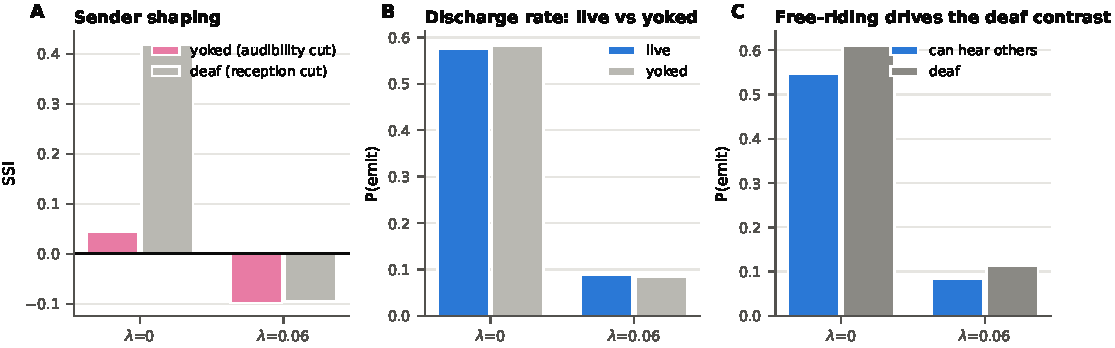
\includegraphics[width=\textwidth]{../figs/fig6_ssi.pdf}
\caption{\textbf{Sender shaping measured with reception held fixed.} (A) SSI from
the yoked contrast, which cuts audibility only, beside the confounded deaf
contrast, which cuts reception. (B) Discharge rate, live versus yoked. (C) The
free-riding effect that drives the deaf contrast: fish that can hear neighbours
discharge less.}
\label{fig:ssi}
\end{figure}

\subsection{A decoupled variable is what lets a social function appear}

A negative result is only as good as the positive control beside it, and to this
point every manipulation has left the discharge welded to its sensory function.
We therefore gave the agents a second variable: a discharge subtype, one bit,
that rides on the pulse---so sending still costs a pulse and still exposes the
fish to predators---but whose value changes nothing about the emitter's own
electric image, nothing about how the pulse illuminates neighbours, and nothing
about detectability. Only the content is decoupled, not the act.

\DECOUPLEDRESULT


\subsection{The same decomposition in a world with no electric fish in it}

If the result is about dual-use action channels rather than about
electroreception, it should reappear wherever an action senses and broadcasts at
once. We built a minimal environment with no fish physics in it: agents forage in
a unit square, and a \textsc{ping} action has exactly the three consequences a
discharge has---it shows the pinger the items near itself, it shows nearby others
the items near \emph{them}, and it is registered by everyone as an event with a
bearing. A weak always-on passive sense means silencing an agent is not the same
as blinding it. The same masks, the same trainer and the same intervention battery
apply unchanged.

The decomposition replicates. Agents that can ping collect \DUFull\ items per
episode against \DUSilent\ for permanently silent ones; muting one agent costs it
\DUTotal\ items, of which \DUPriv\ (\DUPrivFrac\%) is its own lost reafference and
\DUSig\ its lost detectability (Appendix~\ref{app:dualuse}). Pricing the ping
suppresses it from \DUPingLo\ to \DUPingHi. Neither the sign nor the rough
magnitude of the decomposition depends on the electric-fish biophysics; what it
depends on is that one action does two jobs.


\subsection{The regime map, and how far it generalises}

Appendix~\ref{app:regimes} gives the full cost $\times$ predation $\times$
economics grid and the rule-based regime labels. The structure
is orderly, but it is the structure of a probe schedule being turned up and
down: the axes that move are discharge rate and mortality, while the
informational and payoff-relevance axes stay near zero throughout.

\GENERALISATION

\begin{table}[t]
\centering\small
\caption{The muting decomposition across scales and architectures. ``Private share'' is the fraction of the total muting effect attributable to the emitter's own lost reafference.}
\label{tab:gen}
\begin{tabular}{lrrrrr}
\toprule
Condition & seeds & total & $-$reafference & $-$detection & private share \\
\midrule
baseline (4 fish, 60\,cm, 512 steps) & 12 & -0.40 & -0.40 & +0.11 & 101\% \\
2 fish & 6 & -1.66 & -1.58 & -0.02 & 95\% \\
6 fish & 6 & -0.43 & -0.59 & -0.08 & 135\% \\
100\,cm arena & 6 & -0.31 & -0.34 & -0.02 & 107\% \\
1024-step episodes & 6 & -1.10 & -0.92 & +0.08 & 83\% \\
256-unit GRU & 6 & -0.61 & -0.57 & +0.11 & 93\% \\
\bottomrule
\end{tabular}
\end{table}




\section{Discussion}

\paragraph{An effect on a receiver is not a signal.}
The operational definition used by \citet{singh2025active}---an \eod\ that
conspecifics detect and that changes their behaviour---is satisfied in our model
at every metabolic cost we tested, including zero. It is satisfied because the
knollenorgan channel really does carry information and receivers really do
respond to it. Yet the same channel has no detectable consequence for anyone's
payoff: replaying, scrambling or fabricating it moves neither party's return by
an amount we can resolve. We are careful about what that licenses. Our
equivalence tests do not clear the \SI{5}{\percent} margin we set in advance,
because the confidence intervals are wider than the margin; the defensible
statement is \emph{no effect detectable at this sample size}, not demonstrated
equivalence. What makes the negative interpretable is not the width of those
intervals but the assay validation of \S\ref{sec:assay}: the same tests, applied
to a dyad that is communicating by construction, return effects one to two orders
of magnitude larger than anything we see here.

So the strongest defensible form of the claim is this. A system can satisfy the
standard positive-signalling and positive-listening diagnostics without any
detectable payoff relevance and without evidence that production was shaped by
being heard.

Establishing the production-side half of the argument turned out to need more
care than we first gave it. Disabling knollenorgans removes \emph{reception}, so
a hearing/deaf contrast asks whether a fish behaves differently when it can hear
others---not whether it behaves differently when others can hear \emph{it}. Those
are different questions, and the first is contaminated by free-riding: a fish
that can hear its neighbours' probes cuts its own costly sampling, which is what
we in fact observe. The control that isolates being listened to has to hold
reception fixed and cut audibility, which is what our yoked condition does.

\paragraph{The muting confound.}
Silencing a fish is the natural intervention and it is the one available in real
experiments, but it removes three things simultaneously. Our decomposition shows
that the three shares are not merely different in size---they act on different
individuals and in different directions. Losing reafference hurts the muted fish;
losing the illumination it provided hurts its neighbours; losing its detectability
changes how the group is spaced. A single number attributed to ``communication''
averages over all three. The same caution applies to real ablation work: an
\eod-silenced \emph{Gnathonemus} is not a fish with its telephone taken away, it is
a fish that has been blinded and has stopped lighting the room for everyone else.

\paragraph{Cost does not manufacture semantics.}
It is natural to expect that pricing a pulse would turn a probe schedule into an
informative one: a budget has to be spent where it pays, and that allocation
should make the train diagnostic of the emitter's state. That is not what
happens. Across the whole cost range the pulse train becomes rarer and
\emph{less} informative about every target we decoded, and it stays less
informative after normalising per pulse. The learned response to a price is a
lower baseline rate, not a smarter schedule. Whatever costly signalling does in
the classical models
\citep{zahavi1975mate,grafen1990biological,szamado2011cost}, it presupposes a
signal whose honesty is at stake; it does not by itself bring one into being.

What we should not conclude is that a binary pulse leaves no room for a code. A
binary event repeated in continuous time supports a large space of temporal
codes---inter-pulse intervals, bursts, pauses, event-locked patterns---and
mormyrid communication is known to use pulse timing and waveform identity
\citep{baker2013multiplexed,carlson2004stereotyped,hopkins1988neuroethology}. Our
agents \emph{failed to exploit} the temporal code available to them under the
pressures we applied. That is a claim about what learning found, not about what
the channel permits.

\paragraph{Silence tracks the regime, not the moment.}
Cessation of discharge is documented in mormyrids as both predator avoidance and
submissive display \citep{stoddard1999predation,moller1989electric}, and we
expected a momentary version: quiet when the predator is near. It does not appear.
Discharge probability is essentially unchanged by a predator within
\SI{25}{\centi\metre} (\SilenceDangerDiff) and danger is near-undecodable from the
public channel (\DangerAUC\ AUC). Agents lower their \emph{baseline} rate wherever
predators exist, and mortality falls with it, so crypsis works without timing. The
likely reason is sensory asymmetry: our predator hears discharges at
\SI{60}{\centi\metre} but is passively detectable only at \SI{25}{\centi\metre}.

\paragraph{Signalling as a public good and a public hazard.}
Two externalities operate in opposite directions, neither in the reward function:
a discharge illuminates neighbours' worlds, and it also jams their passive sense
and draws an eavesdropping predator toward the group. Cooperative harvesting
sustains a higher rate than competition at matched cost, consistent with the
public-good component being internalised when the harvest is shared. We do not
state that as a mechanism: our interventions found no detectable payoff
consequence of the public channel, so we cannot also claim neighbours benefit
enough from a pulse to explain the rate difference, which may instead reflect
altered encounter distributions or an effect below our resolution.

\paragraph{What the discharge lacks is not a channel.}
The decoupled control was meant to test the hypothesis that dual use is what
blocks signalling: give the fish a variable it can move without degrading its own
sensing, and a social function should appear. It does not. Agents mark half their
discharges with the subtype---the rate an unmodulated bit would give---and
deleting it costs nobody anything in any of the four ecological settings.

Setting that beside the referential assay says what the missing ingredient is.
The assay differs from the foraging world in three ways, and only one of them is
the channel. It also gives the sender information the receiver cannot get for
itself, and it pays both of them when the receiver acts on it. In the foraging
world a fish can find food with its own probe, so a neighbour's private state is
worth very little; there is a channel available and nothing to say over it.
Channel factorisation is plausibly necessary for a signal to become distinct from
a probe, but it is clearly not sufficient. That is a testable prediction for the
biology: electric communication should be elaborated in exactly those contexts
where one fish reliably knows something a conspecific cannot discover
first-hand---dominance status, reproductive state, individual identity---and not
in contexts where both parties can simply sense the world.

\paragraph{Relation to emergent-communication work.}
Most emergent-communication studies equip agents with a dedicated, costless,
otherwise-useless channel \citep{foerster2016learning,mordatch2018emergence,lazaridou2017multi}.
Under those conditions any use of the channel is communicative by construction,
and the interesting question is what code emerges. Electric fish invert the setup:
the channel is a physical act with a large private benefit, and the interesting
question is whether \emph{any} of its use is communicative. We think this is the
more common situation in biology---most signals are thought to be ritualised from
behaviours that originally had other functions---and it is a setting in which the
standard metrics need the production-side test that SSI supplies. Positive
signalling and positive listening are both necessary; neither, nor both together,
is sufficient.

\section{Limitations}

Six bound the claims above and are set out in full in
Appendix~\ref{app:limitations}. The three that matter most: our populations adapt
by policy-gradient learning within a training run, not by an evolutionary outer
loop, so the Sender Shaping Index is a within-lifetime analogue of
\citeauthor{scottphillips2008defining}'s criterion rather than the criterion
itself, and we write \emph{emerge under learning} throughout. Our knollenorgan
channel is all-or-none, as upstream, so graded amplitude signalling is
structurally impossible in the coupled condition, and the decoupled condition
lifts only the crudest version of that restriction --- one bit, not a waveform.
And the equivalence tests do not reach the margin we set in advance; what makes
the nulls interpretable is the assay validation of \S\ref{sec:assay}, not the
width of those intervals.


\small
\bibliographystyle{unsrtnat}
\bibliography{refs}
\normalsize

\clearpage
\appendix
\section*{Appendix}
\addcontentsline{toc}{section}{Appendix}

\section{Numerical validation against the reference implementation}
\label{app:validation}

Every stage of the sensory pipeline is checked against the original NumPy code
in double precision on random scenes (\texttt{scripts/validate\_physics.py}).
Agreement is at floating-point round-off, and the knollenorgan and ampullary
pathways agree bit-for-bit.

% auto-generated by scripts/figures.py
\begin{table}[t]
\centering\small
\caption{Agreement between the GPU reimplementation and the reference NumPy implementation, in double precision on random scenes. Error is the maximum absolute deviation normalised by the largest magnitude present.}
\label{tab:validation}
\begin{tabular}{lr}
\toprule
Stage & Max. relative deviation \\
\midrule
Coulomb field of point charges & $\num{2.3e-15}$ \\
Field of point dipoles & $\num{1.4e-14}$ \\
Field including first-order wall images & $\num{1.9e-15}$ \\
Dipoles induced on conductors & $\num{1.2e-15}$ \\
Charge-limiting of fish body moments & $\num{1.2e-15}$ \\
Corollary-discharge baseline & $\num{1.6e-14}$ \\
Ampullary intrinsic baseline & $\num{1.3e-14}$ \\
Mormyromast, self-image mode & $\num{6.0e-10}$ \\
Mormyromast, collective-sensing mode & $\num{4.9e-11}$ \\
Knollenorgan (conspecific detection) & exact (0) \\
Ampullary (passive DC) & exact (0) \\
\bottomrule
\end{tabular}
\end{table}


\begin{figure}[h]
\centering
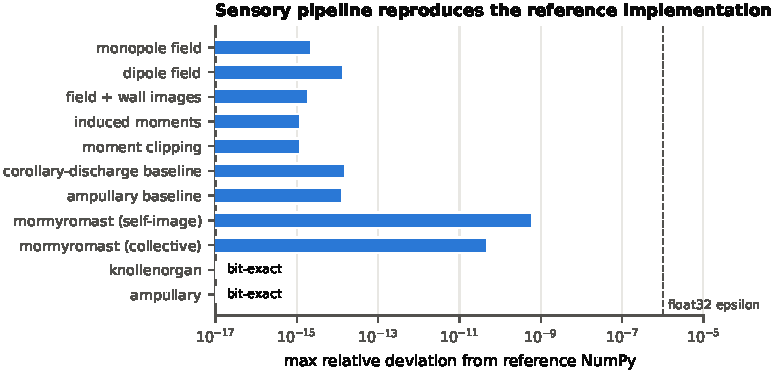
\includegraphics[width=0.62\textwidth]{../figs/fig1_validation.pdf}
\caption{Maximum relative deviation from the reference NumPy implementation over
random scenes, in double precision. Bars at the left edge are exactly zero.}
\label{fig:validation}
\end{figure}

\paragraph{An incidental bug in the reference code.} Its configuration file sets
a wall-reflection coefficient of $0.95$, but \texttt{ElectricScene.\_build\_%
reflections} never forwards it to \texttt{reflect\_sources}, whose default is
$1.0$. The published results therefore use unattenuated first-order images. We
match the code rather than the configuration file; using $0.95$ shifts the
corollary-discharge baseline by $\sim\num{1.4e-6}$ relative and changes ampullary
readings qualitatively, because those are a small difference of large numbers.

\section{Training the three channel conditions from scratch}
\label{app:scratch}

Training is bimodal: a seed either discovers patch foraging or stays near the
floor set by passive sensing alone. A seed counts as converged if it reaches half
the ceiling of its own task family, a criterion applied identically to every
condition within a family; the fraction clearing it is reported as its own
outcome, because conditions that remove sensory channels are not only worse on
average but less reliably learnable.

\begin{figure}[h]
\centering
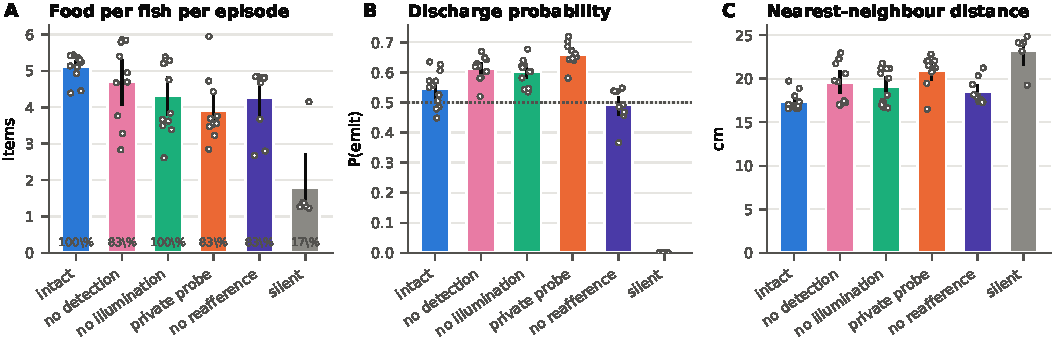
\includegraphics[width=\textwidth]{../figs/fig2_channels_scratch.pdf}
\caption{Removing each consequence of a discharge, trained from scratch. Bars are
means over independent seeds with bootstrap 95\% CIs; points are seeds.
Percentages in (A) give the fraction of seeds reaching the learning criterion.}
\label{fig:scratch}
\end{figure}

\section{Regime classification}
\label{app:regimes}

\begin{figure}[h]
\centering
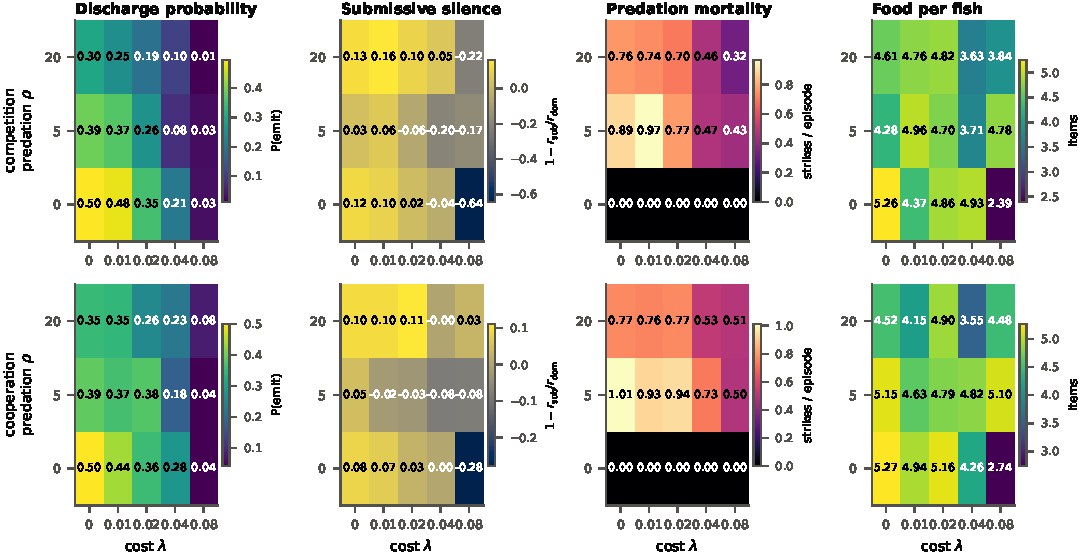
\includegraphics[width=\textwidth]{../figs/fig7_phase_grid.pdf}
\caption{Metabolic cost and eavesdropping predation jointly set discharge policy.
Rows are competitive and cooperative harvests; each cell is a mean over
independent seeds.}
\label{fig:phase}
\end{figure}

\begin{figure}[h]
\centering
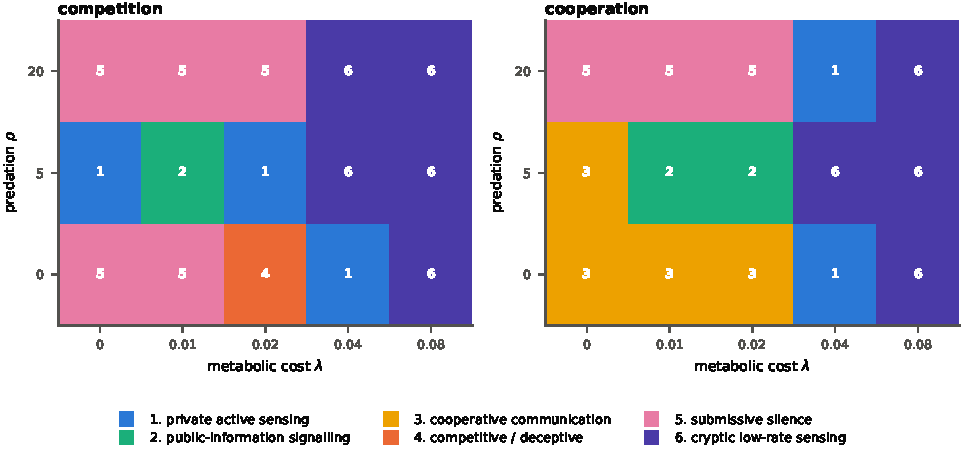
\includegraphics[width=0.92\textwidth]{../figs/fig8_regimes.pdf}
\caption{Rule-based regime labels from the pooled metric vector. Thresholds are
percentiles of each metric's own distribution across the grid rather than
hand-set values, so the boundaries describe a continuum and are not claims about
sharp transitions.}
\label{fig:regimes}
\end{figure}

\section{Limitations in full}
\label{app:limitations}

We list these plainly because several of them bound the claims above.

\begin{enumerate}[leftmargin=1.4em,itemsep=2pt,topsep=2pt]
\item \textbf{Learning is not evolution.} Our populations adapt within a training
      run by policy-gradient learning under a fixed reward. The Scott-Phillips
      criterion refers to evolutionary history, and SSI is a within-lifetime
      analogue: it asks whether the emission policy that learning arrives at
      depends on whether receivers respond. A genuine evolutionary outer loop
      over heritable emission traits would test the criterion directly, and we did
      not run one. We write ``emerge under learning'' throughout rather than
      ``evolve''.
\item \textbf{One arena scale, one group size.} Everything is measured with four
      fish in a $60\times\SI{60}{\centi\metre}$ arena, in which the knollenorgan
      channel at unit gain reaches every conspecific. The range sweep partially
      addresses this, but group size is not varied, and the upstream model
      randomises arena size in a way we deliberately do not.
\item \textbf{Pulses are binary and fixed-amplitude.} Mormyrid electric
      communication uses inter-pulse-interval patterning and species- and
      individual-specific waveform structure
      \citep{baker2013multiplexed,carlson2004stereotyped}; in wave-type
      gymnotiforms, amplitude modulations carry honest size information
      \citep{gavassa2012signal}. Our knollenorgan channel is all-or-none, as
      upstream, so waveform and amplitude signalling are structurally impossible
      in the coupled condition. This is precisely the limitation the decoupled
      condition is designed to lift, and it lifts only the crudest version of it:
      one bit of subtype, not a graded waveform.
\item \textbf{Episodes are short.} 512 steps is about \SI{6}{\second} of fish time.
      Dominance relationships in real fish are established over much longer
      horizons, so the dominance-related results should be read as
      within-encounter, not as stable social structure.
\item \textbf{The metabolic cost is a reward term, not a physiological model.} We
      express cost in reward units and report the fraction of the achieved return
      it consumes so that it can be compared with measured energy budgets, but we
      do not model the electrocyte physiology that sets the true cost, nor its
      dependence on amplitude.
\item \textbf{The predator is a caricature.} It is guided by discharges alone. Real
      electroreceptive predators also use vision, mechanoreception and olfaction,
      so real silence buys less safety than it does here, and the cryptic regime is
      correspondingly easier to reach in our model than in a river.
\item \textbf{Regime labels are a classification imposed on a continuum.} The
      phase diagram is generated by thresholding continuous metrics at percentiles
      of their own pooled distribution. The boundaries are therefore descriptive,
      not sharp transitions, and we make no claim about criticality or
      bifurcation.
\end{enumerate}


\section{Methods}
\label{app:methods}

\subsection{Simulator}

The environment is a GPU reimplementation of the weakly-electric-fish simulator
of \citet{singh2025active}, rewritten so that thousands of independent arenas are
advanced as a single set of tensor operations. All electrostatic constants,
receptor counts, receptor placements, dynamic ranges, transduction functions,
locomotor limits and reward coefficients are transcribed from that codebase; the
differences are enumerated in \S\ref{sec:divergences}.

\paragraph{State and kinematics.}
Each arena holds $F=4$ fish, $N=48$ food items and optionally one predator, in a
\SI{60}{\centi\metre} $\times$ \SI{60}{\centi\metre} rectangular tank with
insulating walls. Fish $i$ has position $\mathbf{x}_i$, heading $\theta_i$ and a
body size $s_i\in[0,1]$ that is fixed within an episode and sets a dominance
rank. The timestep is $\Delta t = 1/83\,\mathrm{s} = \SI{12.05}{\milli\second}$,
matched by the original authors to the social echo-response latency of
\emph{Gnathonemus petersii} \citep{schuster2001count}; episodes last $512$ steps
($\approx\SI{6.2}{\second}$). Motion is first-order in the commanded velocities,
\begin{equation}
\omega_i = u^{\text{turn}}_i \omega_{\max}(1+s_i),\qquad
\mathbf{x}_i \leftarrow \mathbf{x}_i + \hat{u}(\theta_i)\,
  \max(u^{\text{fwd}}_i,0)\, v_{\max}(1+s_i),
\end{equation}
with $v_{\max}=\SI{0.422}{\centi\metre}$ per step and
$\omega_{\max}=\SI{0.0434}{\radian}$ per step, taken from the empirical
percentiles used upstream. A fish whose proposed position would overlap another
fish does not move and receives a collision penalty; walls clamp position without
penalty.

\paragraph{Electric fields.}
All fields are exact Coulomb superposition, with the distance softening
$\varepsilon_m=\SI{e-5}{\metre}$ applied \emph{before} exponentiation exactly as
upstream. A discharging fish carries two monopoles at $\pm\SI{0.5}{\centi\metre}$
along its body axis with charges $\pm q_0$, $q_0=\SI{1.11e-15}{\coulomb}$
\citep{chen2005modeling}:
\begin{equation}
\mathbf{E}_{\text{mono}}(\mathbf{r}) = k\sum_p
  \frac{q_p(\mathbf{r}-\mathbf{r}_p)}{(\lVert\mathbf{r}-\mathbf{r}_p\rVert+\varepsilon_m)^3},
\qquad
\mathbf{E}_{\text{dip}}(\mathbf{r}) = k\sum_d
  \left[\frac{3(\mathbf{p}_d\!\cdot\!\mathbf{u}_d)\mathbf{u}_d}{\lVert\mathbf{u}_d\rVert^5}
        -\frac{\mathbf{p}_d}{\lVert\mathbf{u}_d\rVert^3}\right],
\end{equation}
with $k=\SI{8.99e9}{\newton\metre\squared\per\coulomb\squared}$ and
$\mathbf{u}_d=\mathbf{r}-\mathbf{r}_d$. Fish and food carry permanent intrinsic
dipoles ($\SI{1.11e-23}{}$ and $\SI{1.11e-24}{\coulomb\metre}$). Food items and
non-discharging fish are polarisable insulating spheres,
\begin{equation}
\mathbf{p}^{\text{ind}}_n = 3\varepsilon_0 V_n \chi\, \mathbf{E}(\mathbf{y}_n),
\qquad V_n = \tfrac{4}{3}\pi a_n^3,\quad \chi=-0.5,
\end{equation}
with fish moments capped at $q_0 a_n$. Walls contribute one order of images
across each of the four faces, unattenuated and without sign flip.

\paragraph{Receptors.}
Each fish carries 36 mormyromasts (10 concentrated in a $\pi/3$ chin fovea, 26
spread over the body), 24 ampullary organs and 12 knollenorgans \emph{per
conspecific}. A receptor reads the projection of the local field onto its outward
normal and transduces it by a sign-preserving logarithmic compression into
$[-1,1]$,
\begin{equation}
\hat{s} = \operatorname{sgn}(s)\,
\frac{\log_{10}\operatorname{clip}(|s|,E_{\min},E_{\max}) - \log_{10}E_{\min}}
     {\log_{10}E_{\max}-\log_{10}E_{\min}} .
\end{equation}
Mormyromasts use $[E_{\min},E_{\max}]=[\num{5e-8},\num{5e-2}]\,\si{\volt\per\metre}$
and report the field of the \emph{induced} dipoles alone: the direct discharge
field is cancelled, so what remains is the electric image of objects. Images
carried by a conspecific's discharge rather than one's own are rescaled by
$\num{100}$, as upstream. Ampullary organs
($[\num{2e-10},\num{2e-8}]\,\si{\volt\per\metre}$) sense only the permanent
intrinsic dipoles and are therefore independent of any discharge; a conspecific
discharge degrades them (multiplicative noise fraction rising from $0.05$ to
$0.5$), so emitting jams a neighbour's passive sense. Knollenorgans are
all-or-none: a slot fires with the sign of the local field when
$|s|>\SI{2e-7}{\volt\per\metre}$ (a detection range of $\approx\SI{100}{\centi\metre}$
at unit gain). Crucially, the knollenorgan array is indexed \emph{by emitter}, so
sender identity and bearing are preserved, and each slot carries a noisy scalar
of the emitter's relative body size.

\paragraph{Task and reward.}
Food is distributed in four Gaussian patches ($\sigma=\SI{6}{\centi\metre}$) and
is not replenished. A fish eats an item within \SI{2}{\centi\metre} and $\pm\pi/4$
of its heading; contested items go to the larger fish. The per-step reward is
\begin{equation}
r_i = 10\,n^{\text{eat}}_i
 + \tfrac{d^{\text{prev}}_i-d^{\text{food}}_i}{W+H}
 - 5\,b^{\text{bitten}}_i(1+s_{\text{biter}}-s_i)
 - 0.001\,b^{\text{bite}}_i
 - 0.5\,c^{\text{coll}}_i
 \;\underbrace{-\,\lambda\,e_i}_{\text{new}}
 \;\underbrace{-\,\rho\,k_i}_{\text{new}},
\end{equation}
where $e_i\in\{0,1\}$ indicates a discharge and $k_i$ a predator strike. The first
five terms are upstream's; $\lambda$ (metabolic cost) and $\rho$ (predation) are
introduced here. Under cooperative harvesting a fraction $\alpha$ of each
neighbour's intake is added to $r_i$.

\paragraph{Predators.}
A predator perceives only fish that discharged on the current step and lie within
\SI{60}{\centi\metre}, weights them by $1/(d+1)$, and advances
\SI{0.45}{\centi\metre} toward the loudest. Within \SI{4}{\centi\metre} it strikes
the nearest fish---not necessarily the emitter---and enters a 40-step refractory
period before respawning at a random location. A silent fish is invisible, but a
silent fish beside a discharging neighbour is not safe, so signalling imposes a
risk externality on the group. The predator carries a strong intrinsic dipole and
is therefore detectable passively at $\approx\SI{25}{\centi\metre}$, far inside
the range at which it detects discharges.

\subsection{The channel algebra}
\label{sec:algebra}

A discharge by fish $j$ at time $t$ is routed through three independent binary
masks:
\begin{center}
\begin{tabular}{ll}
\toprule
$V^{\text{self}}_j$ & does $j$'s pulse produce $j$'s own electric image? \\
$V^{\text{illum}}_j$ & does $j$'s pulse produce images on \emph{other} fish's mormyromasts? \\
$V^{\text{det}}_j$ & does $j$'s pulse register on other fish's knollenorgans? \\
\bottomrule
\end{tabular}
\end{center}
Setting all three equal to the emitted action recovers the biological default.
The conditions used here are: \textsc{private} ($V^{\text{illum}}=V^{\text{det}}=0$),
\textsc{cue-only} ($V^{\text{det}}=0$), \textsc{signal-only} ($V^{\text{illum}}=0$),
\textsc{social-only} ($V^{\text{self}}=0$), and \textsc{mute} (all zero, the
upstream intervention). Three further manipulations act on what receivers hear
without changing what the emitter does, so that any change in receiver behaviour
is attributable to the public channel alone:
\begin{itemize}[leftmargin=1.4em,itemsep=1pt,topsep=2pt]
\item \textbf{Phantom.} Receivers perceive discharges from $j$ drawn from an
      exogenous Bernoulli process that $j$ did not choose.
\item \textbf{Replay.} $j$'s public train is replaced by the train the same policy
      produced in a \emph{different arena}. Marginal rate, burst structure and
      inter-pulse-interval statistics are preserved exactly---these are the same
      trains---while the contingency between a pulse and the receiver's current
      world is destroyed. A context-swapped variant pairs each arena with the one
      whose food-proximity time series is most opposite.
\item \textbf{Scrambling.} Timing scrambling circularly shifts each train,
      preserving rate and destroying temporal alignment; identity scrambling
      permutes the knollenorgan slots, preserving rate and timing and destroying
      sender identity.
\end{itemize}

\subsection{Learning}

Agents are trained with recurrent multi-agent PPO
\citep{yu2022surprising,schulman2017proximal} under centralised training with
decentralised execution: one shared actor (2-layer MLP encoder, LayerNorm, $\tanh$,
128 units $\rightarrow$ GRU with 128 units \citep{cho2014learning}) and a
centralised critic that observes all agents' concatenated observations. The action
space is hybrid---two Gaussians for thrust and turn, two Bernoullis for discharge
and bite. Keeping the discharge decision explicitly Bernoulli matters for the
analysis, because its probability is exactly the quantity we intervene on. GAE
\citep{schulman2016high} with $\gamma=0.99$, $\lambda=0.95$; PPO clip $0.2$; 4
epochs, 4 minibatches; Adam at $\num{3e-4}$; 512 parallel arenas; 64-step
truncated BPTT; \SI{18e6}{} agent-steps per run. Every condition is trained from
scratch with independent seeds; \emph{no seed selection of any kind is applied},
and all reported statistics pool over all seeds.

\subsection{Measurement}

\paragraph{Interventional causal influence.}
\citet{jaques2019social} define the influence of agent $j$ on agent $i$ as the KL
divergence between $i$'s policy conditioned on $j$'s actual action and its policy
marginalised over $j$'s alternatives, and estimate it with a learned model of
other agents. Owning the simulator, we evaluate the counterfactual directly:
\begin{equation}
\mathrm{CIE}^{j\to i}_t = \KL\!\left[
  \pi_i\!\left(\cdot \mid h^i_t, o^i_t[\dosim(e_j{=}1)]\right)
  \;\middle\|\;
  \pi_i\!\left(\cdot \mid h^i_t, o^i_t[\dosim(e_j{=}0)]\right)\right],
\label{eq:cie}
\end{equation}
where $o^i_t[\cdot]$ denotes re-rendering $i$'s entire sensory input under the
intervention with the recurrent state $h^i_t$ and every other cause held on its
factual path. The KL is analytic for the factored
Gaussian~$\times$~Bernoulli policy. The null is the same quantity computed between
two re-renderings of the \emph{same} intervention under independent sensory-noise
draws: the divergence the policy shows when nothing about the message changed.

\paragraph{Positive signalling and positive listening.}
Positive signalling \citep{lowe2019pitfalls} is the mutual information between a
window descriptor of the emitter's pulse train (discharge count over 21 steps,
quantised) and the emitter's private state, normalised by the state entropy and
computed \emph{conditionally on} distance-to-nearest-neighbour decile. The
stratification is essential: in a patchy world a fish near a neighbour is also
near food, so an unconditioned mutual information can be manufactured entirely by
geometry. Estimation is plug-in with Miller--Madow bias correction, with a
permutation null. Positive listening is the $L^1$ divergence between the
receiver's factual policy and its policy under a time-shifted message, which
preserves the marginal rate and destroys contingency---the null recommended by
\citet{lowe2019pitfalls} in preference to a silent channel, which is out of
distribution.

\paragraph{Message content.}
What a receiver could recover is decoded \emph{only} from receiver-observable
quantities: the number of pulses it heard from that emitter in a trailing window
and whether it heard anything. Ground-truth state is never given to the decoder.
Targets are the number of live food items within \SI{10}{\centi\metre} of the
emitter, whether the emitter eats within the next 41 steps, emitter body size
(dominance), emitter turn command (intended movement), and whether a predator is
within \SI{25}{\centi\metre} (danger). We report cross-validated $R^2$ or AUC
minus the same quantity computed on time-shifted messages, so that any score
attributable to marginal rate alone is subtracted off.

\paragraph{Sender Shaping Index.}
A signal, on \citeauthor{scottphillips2008defining}'s definition, requires that
production be shaped by its effect on receivers. We train matched populations in a
\emph{hearing} world and a \emph{deaf} world (knollenorgans disabled throughout
training) and compare their emission policies on a common, condition-neutral batch
of observations:
\begin{equation}
\mathrm{SSI} = \frac{\mathbb{E}_{c}\,
  D_{\mathrm{JS}}\!\left[\pi^{\mathcal{H}}_{\text{emit}}(\cdot\mid c)\,\middle\|\,
                          \pi^{\mathcal{D}}_{\text{emit}}(\cdot\mid c)\right]}
{\mathbb{E}_{c}\, D_{\mathrm{JS}}\!\left[\pi^{\text{seed }a}_{\text{emit}}\,\middle\|\,
                          \pi^{\text{seed }b}_{\text{emit}}\right]} - 1 .
\label{eq:ssi}
\end{equation}
The denominator is the within-world seed-to-seed divergence, so $\mathrm{SSI}\le0$
means the emission policy differs no more between worlds than between seeds of the
same world---i.e.\ nobody listening changes nothing, and the pulse is a
\emph{cue}. $\mathrm{SSI}>0$ means production is shaped by reception.

\paragraph{Payoff consequences and the honesty classification.}
Every channel condition is evaluated against the intact channel \emph{paired
within arena}: the two rollouts share the initial food layout and the sensory
noise stream, so differencing removes essentially all layout variance. Confidence
intervals are 2000-sample bootstraps over arenas. Comparing the intact channel
with a rate-matched replay isolates the payoff value of the signal's
\emph{contingency}. Following \citet{maynardsmith2003animal} and
\citet{dawkins1978animal}, a condition is labelled \textsc{communication} when
contingency benefits both parties, \textsc{manipulation} when it benefits the
sender at the receiver's expense, and \textsc{exploited cue} when it benefits the
receiver at the sender's expense.

\subsection{Validation against the reference implementation}
\label{sec:validation}

Every stage of the sensory pipeline is checked against the original NumPy code in
double precision on random scenes (\texttt{scripts/validate\_physics.py}); results
are in Table~\ref{tab:validation}. Agreement is at floating-point round-off, and
the knollenorgan and ampullary pathways agree bit-for-bit.

\subsection{Deliberate divergences from the reference implementation}
\label{sec:divergences}

We record these explicitly because they bear on how far our results transfer.

\begin{enumerate}[leftmargin=1.4em,itemsep=1pt,topsep=2pt]
\item \textbf{Wall-image amplitude.} Upstream's configuration file sets a
      reflection coefficient of $0.95$, but \texttt{ElectricScene.\_build\_reflections}
      never forwards it, so the code that produced the published results uses
      unattenuated images. We match the code, not the configuration file. Using
      $0.95$ instead shifts the corollary-discharge baseline by $\sim\num{1.4e-6}$
      relative and changes ampullary readings qualitatively, because those are a
      small difference of large numbers.
\item \textbf{Fixed arena and episode length.} Upstream samples arena dimensions
      per episode from $[40,300]\,\si{\centi\metre}$ and does not report episode
      length. We fix a $60\times\SI{60}{\centi\metre}$ arena and 512 steps so that
      conditions in a large factorial sweep are exactly comparable. Our
      conclusions are therefore about one arena scale.
\item \textbf{Collision resolution} is synchronous (all fish propose, then all
      resolve) rather than in agent order.
\item \textbf{Network size.} 128-unit GRU rather than 512, and $\num{18e6}$
      agent-steps per run rather than $\num{5e6}$ environment steps, chosen to fit
      \NumRuns\ independent training runs into the compute budget.
\item \textbf{Sensory noise} is present (multiplicative, fractions given above),
      following the upstream code; the upstream paper text describes a noiseless
      model.
\item \textbf{No seed selection.} Upstream selects a single seed (S1) by an
      ethological criterion and reports analyses on it. We pool over all seeds.
\end{enumerate}



\end{document}
